\documentclass[border=2pt]{standalone}
\usepackage[T1]{fontenc}
\usepackage{lmodern}
\usepackage{amsmath}
\usepackage{tikz}
\usetikzlibrary{arrows.meta,positioning,calc,fit}
\begin{document}
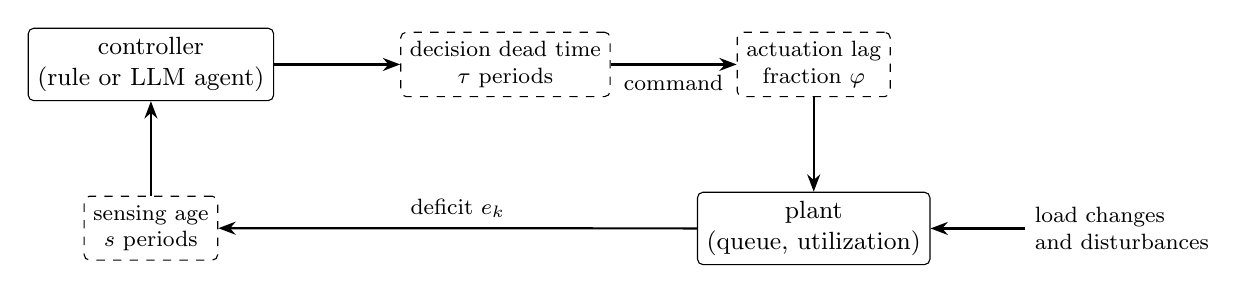
\begin{tikzpicture}[
  node distance=8mm and 16mm,
  box/.style={draw, rounded corners=2pt, minimum height=9mm, minimum width=26mm, align=center, font=\small},
  lag/.style={draw, dashed, rounded corners=2pt, minimum height=7mm, align=center, font=\footnotesize},
  arr/.style={-{Stealth[length=2.2mm]}, thick}]
  \node[box] (ctl) {controller\\(rule or LLM agent)};
  \node[lag, right=of ctl] (dead) {decision dead time\\$\tau$ periods};
  \node[lag, right=of dead] (act) {actuation lag\\fraction $\varphi$};
  \node[box, below=12mm of act] (plant) {plant\\(queue, utilization)};
  \node[lag, below=12mm of ctl] (sense) {sensing age\\$s$ periods};
  \draw[arr] (ctl) -- (dead);
  \draw[arr] (dead) -- node[below, font=\footnotesize]{command} (act);
  \draw[arr] (act) -- (plant);
  \draw[arr] (plant) -- node[above, font=\footnotesize]{deficit $e_k$} (sense);
  \draw[arr] (sense) -- (ctl);
  \node[font=\footnotesize, align=left, anchor=west] (dist) at ($(plant.east)+(12mm,0)$) {load changes\\and disturbances};
  \draw[arr] (dist.west) -- (plant.east);
\end{tikzpicture}
\end{document}
